\documentclass[12pt]{article}
\usepackage[utf8]{inputenc}
\usepackage[english]{babel}
\usepackage[table,xcdraw]{xcolor}
\usepackage{hyperref}
\usepackage{float}
\usepackage{amsmath}
\usepackage{mathtools}
\usepackage{tikz}
\usepackage{pgfplots}
\usepackage{blindtext}

\pgfplotsset{compat=1.14} % Disable-lint

\hypersetup{%
	colorlinks,
	citecolor=black,
	filecolor=black,
	linkcolor=black,
	urlcolor=black
}

\usepackage[backend=biber,style=authoryear]{biblatex}
\usepackage[newfloat]{minted}
\usemintedstyle{vs}
\usepackage{csquotes}
\usepackage{caption}
\usepackage{booktabs}


\graphicspath{ {images/} }

\newcommand\tab[1][1cm]{\hspace*{#1}}
\SetupFloatingEnvironment{listing}{name=Code example}
\definecolor{bg}{rgb}{0.95,0.95,0.95}
\newenvironment{code}{\captionsetup{type=listing}}{}

\newcommand\codeblock[3]{%
\begin{code}
	\caption{#3}
	\inputminted[%
	    mathescape,
	    linenos,
	    numbersep=5pt,
	    tabsize=4,
	    label=Helloworld,
	    bgcolor=bg,
	    breaklines%
	]{TypeScript}{#1}
\label{#2}
\end{code}
}

\newcommand\Code[1]{\texttt{#1}}


\addbibresource{sample.bib}

\begin{document}

\begin{titlepage}
	\centering
	\vspace{2cm}
	{\Huge Software implementations and analysis of three voting systems\par}
	\vspace{0.6cm}
	{\LARGE Adrian Salamon\par}
	\vspace{0.6cm}
	{\Large Kungsholmens gymnasium\par}
	\vspace{0.4cm}
	{\large Senior thesis\par}
	\vspace{0.6cm}
	
\includegraphics[width=0.3\textwidth]{kg}\par\vspace{1cm}
	\vspace{4cm}
	\vfill
	Supervised by: \par
	Maja Kankaanranta

	\vfill

	% Bottom of the page
	{\large \today\par}
\end{titlepage}


\pagebreak

\begin{abstract}
	The abstract text goes here.
\end{abstract}

\pagebreak

\tableofcontents

\pagebreak

\section{Introduction}
\subsection{Background}
Taking a collective decision as a population is difficult. To solve this issue, voting systems with defined rules are used. They are used to show common preferences within a population, for example what politician a population wants to see elected. Several types of systems have been designed and there are a myriad of variations of those systems. They range from simple methods such as “most votes win” to complex processes that can only be practically carried out by a computer. However, practically all voting systems are algorithmic in nature, which makes them interesting to study for both Computer Scientists and Mathematicians. When deciding on what systems that shall be used, it is useful to know what differences and similarities they have.
\subsection{Purpose}
The purpose of this essay is to evaluate differences and similarities in terms of election results in three different voting systems: Single Transferable Vote (STV), First-Past-The-Post (FPTP) and the Schulze Method. This paper will only be examining and discussing differences and similarities in the results of the methods, not touching on how practically feasible the methods might be in actual election.
\pagebreak
\section{Theory}
Theory will be here some day
\pagebreak
\section{Methodology}
All voting methods have been implemented in Typescript – mostly due to the author having previous experience with JavaScript. Typescript is a superset of JavaScript with multiple extra features. Most importantly Typescript has optional static type checking. Sample code in typescript can be seen in code example \ref{lst:typescript example}.
\codeblock{code/typescriptexample.ts}{lst:typescript example}{Basic Typescript syntax}
\subsection{Modeling test data}
In order to test the methods and their implementations, test data is needed. There are cases where extensive election data is published, such as in Maltese elections, but full ballot data, which is needed for the implementations has not been found. Instead, the implementations will be tested with data generated from a simple computer algorithm. The algorithm used in this paper is highly primitive, as modeling preferences within a population is far beyond this paper. The full ballot generation program can be found in the \Code{/generator/} folder. The goal of the program is to produce ballots that rank every candidate in order of preference (see figure \ref{fig:stv ballot} on page \pageref{fig:stv ballot}). The program represents each voter in a population as belonging to a certain ideology. Each ideology has has a list of weighted preferences indicating how a voter for this ideology is likely to vote. The weighed preferences are generated via an abstraction. A single configuration object is used to create all ideologies.
\codeblock{code/generator/ideologyConfig.ts}{lst:ideology configuration}{Configuration object for creating ideologies}
The program then works via 4 major steps:
\begin{enumerate}
	\item It relates each candidate to an ideology based on the size of the ideology. A larger ideology has more candidates.
	\item It assigns a base size for each candidate. Each ideology has a different spread of votes generated by a negative exponential function with a different constant. The size of each candidate is then multiplied with the size of their ideology and normalized. This gives a base size of all candidates.
	\item Based on the base size of each candidate, a probability-list of voting for each candidate is created for every ideology. An ideology's probability-list represents how a voter aligned the ideology is expected to vote.
	\item It creates a certain number of individual ballots. Each ballot is given an ideology and creates its own list preferences based via weighted random number generation according to the probability-list of the assigned ideology.
\end{enumerate}
The output of the program is a set of ballots, where each ballot is an ordered set of preferences. The implementation is highly arbitrary and all constants in the program even more so. However, expanding on the generator program would be beyond the scope of this project. The program works in that it is possible to control variables to test for different election scenarios.
\subsection{Constructing test scenarios}
Constructing test scenarios is difficult task. Due to there being so many variables both in real elections and the simulated elections in the generator program, it makes it practically impossible to control all variables. Instead, 3 arbitrary test scenarios will be used. The election will be simulated 1000 times for each scenario and the election data will then run through the different voting methods and the results will be compared. The simulation scenarios are arbitrary but should allow for comparison of the different voting methods. All simulations will have 3 ideologies and 500 voters.
\subsubsection{Scenario 1}
The scenario is built around electing one candidate out of eight. The spread of votes within ideologies is flat and all ideologies are "weak". This means that the general spread of votes will be even. An example of the distribution of first-preference votes generated in this scenario can be seen in figure \ref{fig:example of scenario 1}. The full configuration object can be seen in code example \ref{lst:scenario 1}.
\codeblock{code/generator/scenario1.ts}{lst:scenario 1}{Configuration object for scenario 1}
\begin{figure}[H]
	\centering
	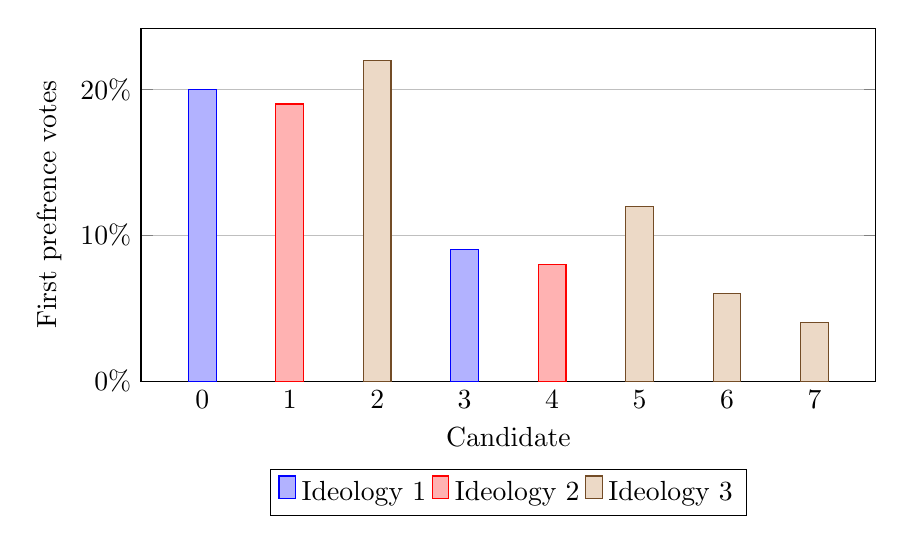
\begin{tikzpicture}
		\begin{axis}[
			ybar stacked,
			width = 0.9\textwidth,
			height = 0.5\textwidth,
			legend style={at={(0.5,-0.25)},
			anchor=north,legend columns=-1},
      x tick style = transparent,
			ylabel = {First prefrence votes},
			xlabel = {Candidate},
			ymajorgrids = true,
      ymin = 0,
			yticklabel={\pgfmathprintnumber\tick\%}
      ]
			\addplot coordinates
			{(0, 20)(1, 0)(2, 0)(3, 9)(4, 0)(5, 0)(6, 0)(7, 0)};
			\addplot coordinates
			{(0, 0)(1, 19)(2, 0)(3, 0)(4, 8)(5, 0)(6, 0)(7, 0)};
			\addplot coordinates
			{(0, 0)(1, 0)(2, 22)(3, 0)(4, 0)(5, 12)(6, 6)(7, 4)};
			\legend{Ideology 1, Ideology 2, Ideology 3}
		\end{axis}
	\end{tikzpicture}
	\caption{Example distribution of first-preference votes in scenario 1}
	\label{fig:example of scenario 1}
\end{figure}
\subsubsection{Scenario 2}
The second scenario elects 3 candidates out of 9 total. It features a normal spread of votes between candidates. An example distribution of first-preference votes generated in this scenario can be seen in figure \ref{fig:example of scenario 2}. The full configuration can be seen in code example \ref{lst:scenario 2}.
\codeblock{code/generator/scenario2.ts}{lst:scenario 2}{Scenario 2}
\begin{figure}[H]
	\centering
	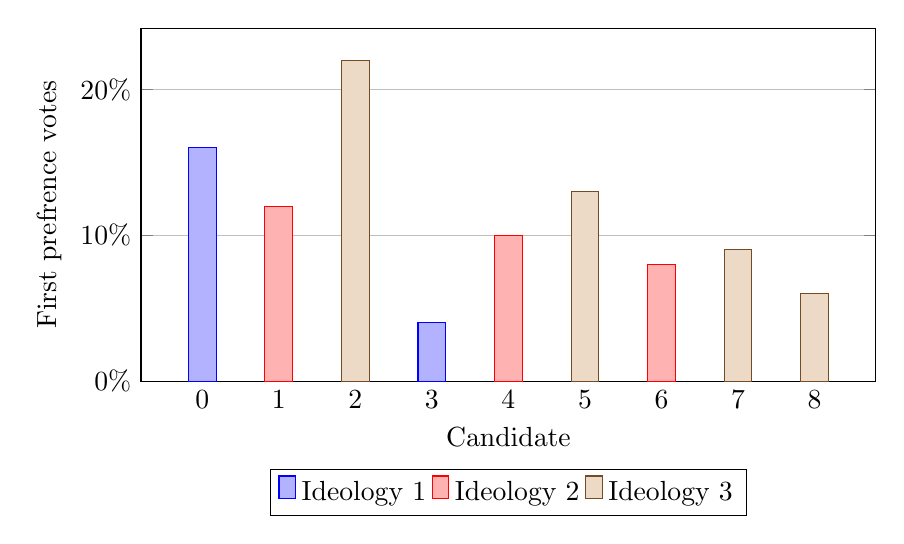
\begin{tikzpicture}
		\begin{axis}[
			ybar stacked,
			width = 0.9\textwidth,
			height = 0.5\textwidth,
			legend style={at={(0.5,-0.25)},
			anchor=north,legend columns=-1},
      x tick style = transparent,
			ylabel = {First prefrence votes},
			xlabel = {Candidate},
			ymajorgrids = true,
      ymin = 0,
			yticklabel={\pgfmathprintnumber\tick\%}
      ]
			\addplot coordinates
			{(0, 16)(1, 0)(2, 0)(3, 4)(4, 0)(5, 0)(6, 0)(7, 0)(8, 0)};
			\addplot coordinates
			{(0, 0)(1, 12)(2, 0)(3, 0)(4, 10)(5, 0)(6, 8)(7, 0)(8, 0)};
			\addplot coordinates
			{(0, 0)(1, 0)(2, 22)(3, 0)(4, 0)(5, 13)(6, 0)(7, 9)(8, 6)};
			\legend{Ideology 1, Ideology 2, Ideology 3}
		\end{axis}
	\end{tikzpicture}
	\caption{Example distribution of first-preference votes in scenario 2}
	\label{fig:example of scenario 2}
\end{figure}
\subsubsection{Scenario 3}
The second scenario elects 3 candidates out of 9 total. It features a steep spread of votes between candidates. An example distribution of first-preference votes generated in this scenario can be seen in figure \ref{fig:example of scenario 3}. The full configuration can be seen in code example \ref{lst:scenario 3}.
\codeblock{code/generator/scenario3.ts}{lst:scenario 3}{Scenario 3}
\begin{figure}[H]
	\centering
	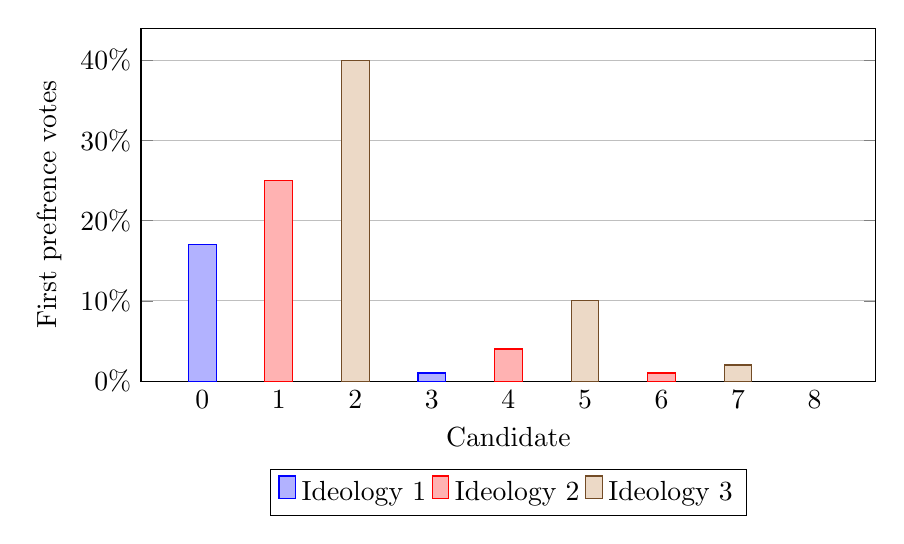
\begin{tikzpicture}
		\begin{axis}[
			ybar stacked,
			width = 0.9\textwidth,
			height = 0.5\textwidth,
			legend style={at={(0.5,-0.25)},
			anchor=north,legend columns=-1},
      x tick style = transparent,
			ylabel = {First prefrence votes},
			xlabel = {Candidate},
			ymajorgrids = true,
      ymin = 0,
			yticklabel={\pgfmathprintnumber\tick\%}
      ]
			\addplot coordinates
			{(0, 17)(1, 0)(2, 0)(3, 1)(4, 0)(5, 0)(6, 0)(7, 0)(8, 0)};
			\addplot coordinates
			{(0, 0)(1, 25)(2, 0)(3, 0)(4, 4)(5, 0)(6, 1)(7, 0)(8, 0)};
			\addplot coordinates
			{(0, 0)(1, 0)(2, 40)(3, 0)(4, 0)(5, 10)(6, 0)(7, 2)(8, 0)};
			\legend{Ideology 1, Ideology 2, Ideology 3}
		\end{axis}
	\end{tikzpicture}
	\caption{Example distribution of first-preference votes in scenario 3}
	\label{fig:example of scenario 3}
\end{figure}
\begin{figure}[H]
	\centering
	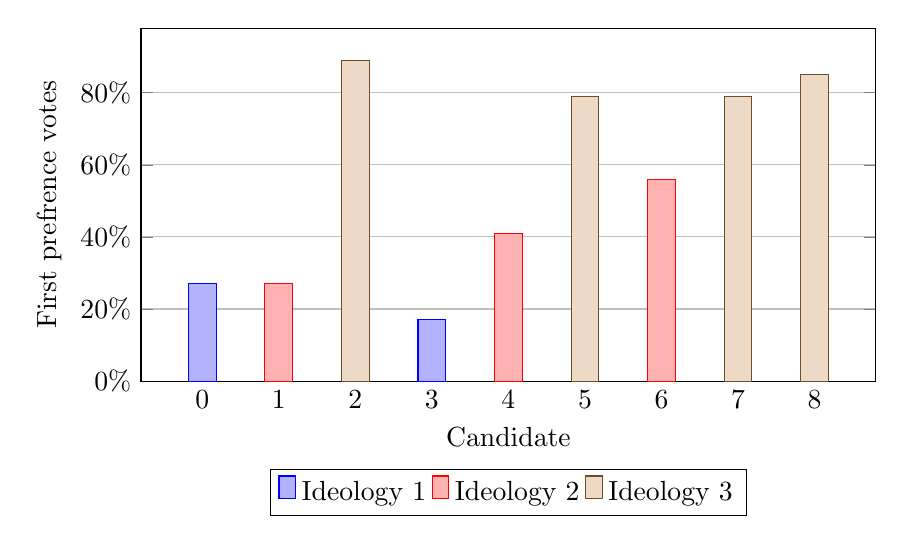
\begin{tikzpicture}
		\begin{axis}[
			ybar stacked,
			width = 0.9\textwidth,
			height = 0.5\textwidth,
			legend style={at={(0.5,-0.25)},
			anchor=north,legend columns=-1},
      x tick style = transparent,
			ylabel = {First prefrence votes},
			xlabel = {Candidate},
			ymajorgrids = true,
      ymin = 0,
			yticklabel={\pgfmathprintnumber\tick\%}
      ]
			\addplot coordinates
			{(0, 27)(1, 0)(2, 0)(3, 17)(4, 0)(5, 0)(6, 0)(7, 0)(8, 0)};
			\addplot coordinates
			{(0, 0)(1, 27)(2, 0)(3, 0)(4, 41)(5, 0)(6, 56)(7, 0)(8, 0)};
			\addplot coordinates
			{(0, 0)(1, 0)(2, 89)(3, 0)(4, 0)(5, 79)(6, 0)(7, 79)(8, 85)};
			\legend{Ideology 1, Ideology 2, Ideology 3}
		\end{axis}
	\end{tikzpicture}
	\caption{Example distribution of first-preference votes in scenario 4}
	\label{fig:example of scenario 4}
\end{figure}



\pagebreak
\section{Specification of voting methods}
\subsection{First-past-the-post}
\subsubsection{Description}
The first-past-the-post voting method is a method designed for electing one or several candidates out of a set of candidates. Each voter has one (1) vote which may be allocated to any candidate. In a first-past-the-post election the N candidates with most votes get elected.
\subsubsection{Justification}
The method is simple and can easily be understood. The first-past-the-post method is widely used in for example the United Kingdom and United States. Comparisons with this method can also be easily made.
\subsubsection{Pseudocode}
let $V$ be the set of votes with $V_{i}$ being the number of votes for candidate $i$ \\
let $N$ be number of candidates to be elected \\
sort $V$ based on $V_{i}$\\
slice $V$ between $0$ and $N$
\subsubsection{Implementation}
The first-past-the-post program is implemented in a single file. The inputs of the program can be seen in code example \ref{lst:fptp inputs}.
\codeblock{code/fptp/inputs.ts}{lst:fptp inputs}{Inputs for FPTP program}
The ballot data is first mapped to only include first preferences. Then the algorithm loops over the ballots and gets the sum of votes for each candidate. This process is shown in code example \ref{lst:fptp processing}.
\codeblock{code/fptp/processing.ts}{lst:fptp processing}{Processing and formatting of data}
The results array is sorted and sliced to only include the $N$ candidates with most votes as seen in code example \ref{lst:fptp result calculation}.
\codeblock{code/fptp/result.ts}{lst:fptp result calculation}{Finding and returning winning candidates}
\subsection{Single transferable vote}
\subsubsection{Description}
The Single Transferable Vote method is a more complicated algorithm than the first-past-the-post method. Voters are given ballots where they are supposed to rank candidates in order. The specific rules for if you need to rank all candidates or rank several candidates at the same value not can vary. For the sake of simplicity, in this implementation, all candidates must be ranked at unique and linear values. An example of a ballot can be seen in figure \ref{fig:stv ballot}.	This means that there is more data available for determining the result of the election which the method can take advantage of. Votes are, if needed, transferred between choices within a ballot, hence the name Single Transferable Vote. The method relies on the concept of a quota, the number of votes you need to be elected. The Droop-Quota, defined as $(\frac{\text{total valid poll}}{\text{seats} + 1})+1$, is often used. If a candidate receives equal or more votes than the quota, he/she is elected. If the number of votes exceed the quota, a fraction of the votes are transferred to the next choice on the ballots that voted for the elected candidate. This process is repeated until there are no candidates with more votes than the quota. If there still are seats yet to be filled, the candidate with fewest votes is eliminated and his/her votes are transferred to the next choice on those ballots. This process is repeated until all seats are filled. The process can become quite complex with many ballots and transferring fractional votes. A computer is therefore essential in order to resolve large scale elections.
\begin{figure}
	\centering
	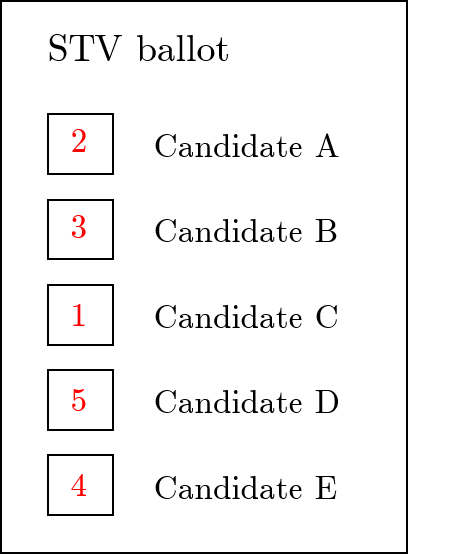
\includegraphics[height=140px]{ballot}
	\caption{Sample STV ballot}
	\label{fig:stv ballot}
\end{figure}
\subsubsection{Justification}
STV is an established voting method in use in several countries. It is used for parliamentary elections in Ireland, Malta and Australia as well as being used in local and regional elections across the world.
\subsubsection{Pseudocode}
\label{alg:stv psuedocode}
let $quota$ be the quota \\
let $seats$ be the number of seats \\
let $winners$ be the list of elected candidates \\
let $votes$ be the set of votes with $votes_{i}$ signifying votes for candidate $i$\\
while $\left\vert{winners}\right\vert < seats$\\
\tab if any candidate $i \notin winners$ and $votes_{i} \geq quota$ \\
\tab\tab add $i$ to $winners$ \\
\tab\tab continue \\
\tab end if \\
\tab if any candidate $i$ where $votes_{i} > quota$\\
\tab\tab multiply $votes_{i}$ with $(1 - \frac{\text{surplus votes}_{i}}{votes_{i}})$ \\
\tab\tab multiply next preferences for $votes_{i}$ with $\frac{\text{surplus votes}_{i}}{votes_{i}}$ and \\ \tab\tab distribute into $votes$\\
\tab\tab continue \\
\tab end if \\
\tab if $\left\vert{votes}\right\vert = seats$ \\
\tab\tab add all $votes \notin winners$ to $winners$ \\
\tab\tab continue \\
\tab end if \\
\tab $k \coloneqq$ index of smallest $votes_{i}$ \\
\tab eliminate $votes_{k}$ and distribute all next-preference votes for candidate $k$ \tab into $votes$\\
end while
\subsubsection{Implementation}
The single transferable vote algorithm uses a tree structure to represent the state of the election. Every candidate is a top-level node with an attribute showing the number of current votes for the candidate. Each node has child nodes representing the next preferences of the voters for that particular candidate, see figure \ref{fig:tree structure}. It is easy to manipulate branches via recursion. Merging and multiplying branches is used when transferring votes from one candidate node to another. A candidate node is a Typescript class. It can be found in the \Code{stv/candidate.ts} file and has the following properties and functions:
\begin{figure}
	\centering
	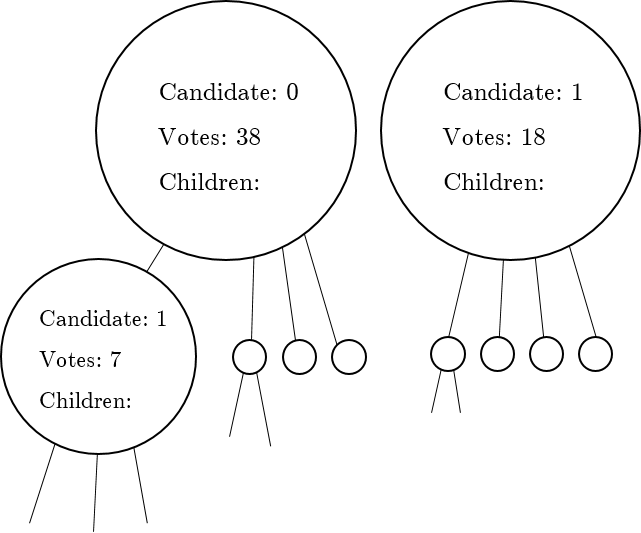
\includegraphics[height=200px]{Tree}
	\caption{Simplified and shortened version of the tree structure. Each candidate is a top-level node with children, signifying the preferences of the voters for that candidate.}
	\label{fig:tree structure}
\end{figure}
\codeblock{code/stv/candidateNode.ts}{lst:stv candidate node}{The CandidateNode class}
With the \Code{add()} and \Code{multiply()} functions it is possible to recursively modify branches. There are two different manipulations that need to be preformed on the tree: transferring surplus votes and eliminating candidates. Both functions rely on the \Code{distribute()} function which is used to distribute a set of nodes onto the tree.
\codeblock{code/stv/distribute.ts}{lst:stv distribute function}{The distribute function}
In order to eliminate and transfer surplus votes from any candidate node $A$, the children of $A$ are passed into the distribute function. In the case of transferring surplus votes, the votes for each child node is first multiplied by $\frac{\text{surplus votes}}{\text{total votes}}$ as outlined in the pseudocode in section \ref{alg:stv psuedocode}. The full source code for functions that manipulate the tree structure can be found in \Code{/stv/tree.ts}.

The main process of the program is found in the \Code{stv/election.ts} file and runs the process defined in the pseudocode in section \ref{alg:stv psuedocode} on page \pageref{alg:stv psuedocode}.

\subsection{Schulze}
\subsubsection{Description}
The Schulze Method is a method used mainly to determine results in a single-winner election but can also be used to provide rankings and elect multiple candidates in a single election. Ballots are identical to those of the single transferable vote, see figure \ref{fig:stv ballot} on page \pageref{fig:stv ballot}. The method is compliant with the Condorcet Criterion, which means that if there is a candidate who the majority prefers in a pairwise comparison with every other candidate, that candidate wins. As mentioned, this method relies on comparing the preferences of every candidate to one another as shown in table \ref{tab:pairwise comparison matrix}. If there is a Condorcet winner the process is simple: declare the Condorcet winner a winner and run another iteration without that candidate. Repeat this process until all seats are filled. However, there can be Condorcet ties, where there is no Condorcet winner. There are multiple ways of resolving the tie, one of them being the Schulze Method.

The Schulze Method resolves ties by investigating possible paths between candidates. For example, if out of a total of 50 ballots 30 ballots prefer $B>A$, 28 ballots prefer $A>C$ and 27 ballots prefer $C>B$, a path from $A$ to $B$ can be created by going $A \rightarrow C \rightarrow B$. The path is said to have the $strength$ of the weakest link in the path. In this example, the path strength between A and B is 27 due to the link between $C$ and $B$ having a strength of 27. There may be several paths between two candidates and the goal of the process is to find the strongest path between any candidate $A$ and $B$, written as $p[A,B]$. By finding the strongest path between all nodes a result can be obtained where $p[X,Y] \geq p[Y,X]$ which means that candidate $X$ wins. The Schulze Method also provides a linear ranking between all candidates, for example that $E > B > A > C > D$. By selecting the $N$ top candidates you can use the method for a multi-seat election. As the process can become very complex as the number of candidates grow, a computer is needed to resolve large elections.

The difficult problem in this method is finding the strongest path between candidates. The problem is called the widest path problem in graph theory. An efficient and relatively simple way to compute this problem is via the Floyd-Warshall algorithm which is used in the implementation. See \ref{lst:schulze algorithm} for the full algorithm.

\begin{table}
\centering
\caption{Pairwise comparison matrix used in the Schulze method. For example, 17 ballots prefer $A>B$ and 33 ballots prefer $B>A$.}
\begin{tabular}{l|c|c|c|c|c|}
\cline{2-6}
 & \multicolumn{1}{l|}{A} & \multicolumn{1}{l|}{B} & \multicolumn{1}{l|}{C} & \multicolumn{1}{l|}{D} & \multicolumn{1}{l|}{E} \\ \hline
\multicolumn{1}{|l|}{A} & \cellcolor[HTML]{9B9B9B} & \cellcolor[HTML]{FFDDDD}17 & \cellcolor[HTML]{FFDDDD}14 & \cellcolor[HTML]{DDFFDD}35 & \cellcolor[HTML]{DDFFDD}30 \\ \hline
\multicolumn{1}{|l|}{B} & \cellcolor[HTML]{DDFFDD}33 & \cellcolor[HTML]{9B9B9B} & \cellcolor[HTML]{FFDDDD}24 & \cellcolor[HTML]{DDFFDD}47 & \cellcolor[HTML]{DDFFDD}36 \\ \hline
\multicolumn{1}{|l|}{C} & \cellcolor[HTML]{DDFFDD}36 & \cellcolor[HTML]{DDFFDD}26 & \cellcolor[HTML]{9B9B9B} & \cellcolor[HTML]{DDFFDD}40 & \cellcolor[HTML]{DDFFDD}42 \\ \hline
\multicolumn{1}{|l|}{D} & \cellcolor[HTML]{FFDDDD}15 & \cellcolor[HTML]{FFDDDD}3 & \cellcolor[HTML]{FFDDDD}10 & \cellcolor[HTML]{9B9B9B} & \cellcolor[HTML]{FFDDDD}18 \\ \hline
\multicolumn{1}{|l|}{E} & \cellcolor[HTML]{FFDDDD}20 & \cellcolor[HTML]{FFDDDD}14 & \cellcolor[HTML]{FFDDDD}8 & \cellcolor[HTML]{DDFFDD}32 & \cellcolor[HTML]{9B9B9B} \\ \hline
\end{tabular}
\label{tab:pairwise comparison matrix}
\end{table}
\subsubsection{Justification}
The Schulze method is used by multiple organizations around the world. It has been used by various software organizations such as The Wikimedia Foundation, The Debian Project and Ubuntu. It is also used by political parties such as the Pirate Party in Sweden and various other countries. The process also differs greatly in both method and implementation from the two other voting methods used in this paper.
\subsubsection{Pseudocode}
\label{alg:schulze psuedocode}
let $d[i,j]$ be the number of ballots that prefer candidate $i$ to candidate $j$\\
let $p[i,j]$ be the strength of the strongest path from candidate $i$ to candidate $j$\\
for $i$ from 1 to $C$\\
\tab for $j$ form 1 to $C$\\
\tab\tab if ($i \ne j$)\\
\tab\tab\tab if ($d[i,j] > d[j,i]$)\\
\tab\tab\tab\tab $p[i,j] \coloneqq d[i,j]$\\
\tab\tab\tab else\\
\tab\tab\tab\tab $p[i,j] \coloneqq 0$\\
\tab\tab\tab end if \\
\tab\tab end if \\
\tab end for \\
end for\\
for $i$ from 1 to $C$\\
\tab for $j$ form 1 to $C$\\
\tab\tab if ($i \ne j$)\\
\tab\tab\tab for $k$ from 1 to $C$\\
\tab\tab\tab\tab if ($i \ne k \text{ and } j \ne k$)\\
\tab\tab\tab\tab\tab $p[j,k] \coloneqq \text{max }(p[j,k], \text{ min }(p[j,k], p[i,k]))$\\
\tab\tab\tab\tab end if \\
\tab\tab\tab end for \\
\tab\tab end if \\
\tab end for \\
end for\\
\subsubsection{Implementation}
The Schulze Method is implemented within the file \Code{schulze/index.ts}. It takes two inputs: a list of ballots and the number of seats to be elected. A ballot is an ordered list of candidates. The output of the program is a list of winners. The program first creates the matrices for both the preferences and paths between candidates.
\codeblock{code/schulze/maps.ts}{lst:schulze maps}{Data representation}
The program then runs the algorithm outlined in the pseudocode in section \ref{alg:schulze psuedocode}.
\codeblock{code/schulze/algorithm.ts}{lst:schulze algorithm}{Main algorithm}
\section{Evaluation of results}
\subsection{Scenario 1}
Scenario 1 featured 8 candidates where one was to be elected. Vote spread was flat, meaning that votes tend to be diverse in their preferences. This means that there is not an obvious winner present. This can be seen from the first-preference votes in the scenario seen in figure \ref{fig:example of scenario 1}. The full result in this scenario can be seen in figure \ref{fig:scenario 1 results}. The outlier in this scenario seems to be the fptp method, electing candidate 0 more often than both other methods. Key metrics for the results in this scenario can be found in table \ref{tab:scenario 1 result}. Although the misrepresentation metric is not entirely accurate, especially when few seats are elected, it shows that fptp is not entirely representative. The STV and Schulze method seem to return very similar results.
\begin{figure}
	\centering
	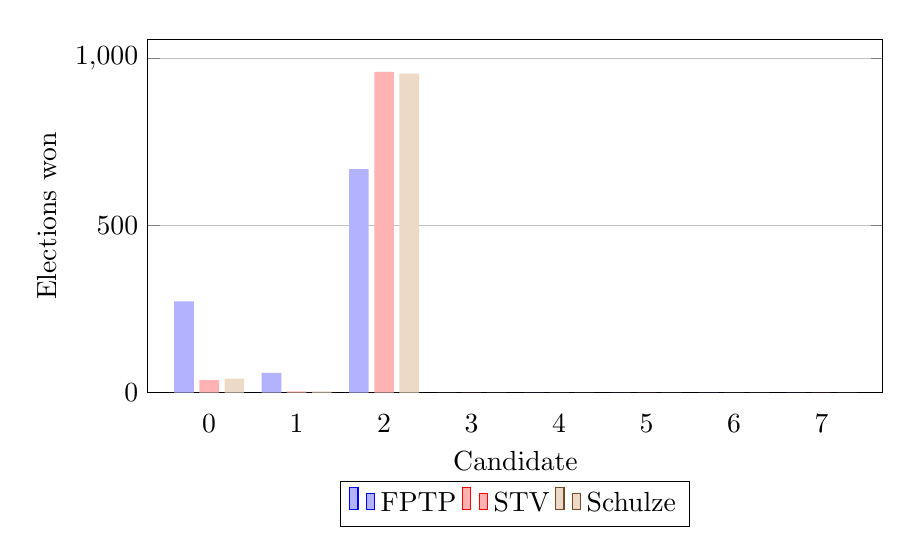
\begin{tikzpicture}
		\begin{axis}[
			ybar,
			width = 0.9\textwidth,
			height = 0.5\textwidth,
			legend style={at={(0.5,-0.25)},
			anchor=north,legend columns=-1},
      x tick style = transparent,
			ylabel = {Elections won},
			xlabel = {Candidate},
			ymajorgrids = true,
			every axis plot/.append style={draw=none,fill,no markers},
      ymin = 0,
			symbolic x coords={0,1,2,3,4,5,6,7,8},
			bar width=0.25cm
      ]
			\addplot coordinates
			{(0, 273)(1, 59)(2, 668)(3, 0)(4, 0)(5, 0)(6, 0)(7, 0)};
			\addplot coordinates
			{(0, 37)(1, 4)(2, 959)(3, 0)(4, 0)(5, 0)(6, 0)(7, 0)};
			\addplot coordinates
			{(0, 42)(1, 4)(2, 954)(3, 0)(4, 0)(5, 0)(6, 0)(7, 0)};
			\legend{FPTP, STV, Schulze}
		\end{axis}
	\end{tikzpicture}
	\caption{Results in scenario 1}
	\label{fig:scenario 1 results}
\end{figure}

\begin{table}
\centering
\caption{Key metrics for result in scenario 1}
\label{tab:scenario 1 result}
\begin{tabular}{@{}lccc@{}}
\toprule
Method & Standard deviation & Misrepresentation & Most likely winners \\ \midrule
FPTP & 223 & 67\% & 2 \\
STV & 315 & 7\% & 2 \\
Schulze & 313 & 9\% & 2 \\ \bottomrule
\end{tabular}
\end{table}
% [ 223.39259164082, 315.44928276983, 313.6271671906]
\subsection{Scenario 2}
Scenario 2 featured 9 candidates of which 3 were to be elected. The distribution of votes was "normal", and as seen in figure \ref{fig:example of scenario 2}, the election is very close with many candidates having a similar percentage of first-preference votes. The results obtained in scenario 2 are very interesting. FPTP tended to underrepresent candidate 1, and elected a candidate from ideology 2 only in 28\% of elections, despite the ideology theoretically having 30\% of popular support. The Schulze method also tended to underrepresent ideology 2. It instead overrepresented ideology 2, electing 3 candidates of ideology 2 in 50\% of elections. This indicates that the Schulze method is not a representative method in a multi-seat election. The STV result showed less misrepresentation than the FPTP result, which was to be expected since the method has access to more data of any voter's preferences. The results in scenario 2 can be observed in figure \ref{fig:scenario 2 result} and the key metrics can be seen in table \ref{tab:scenario 2 result}.
\begin{figure}
	\centering
	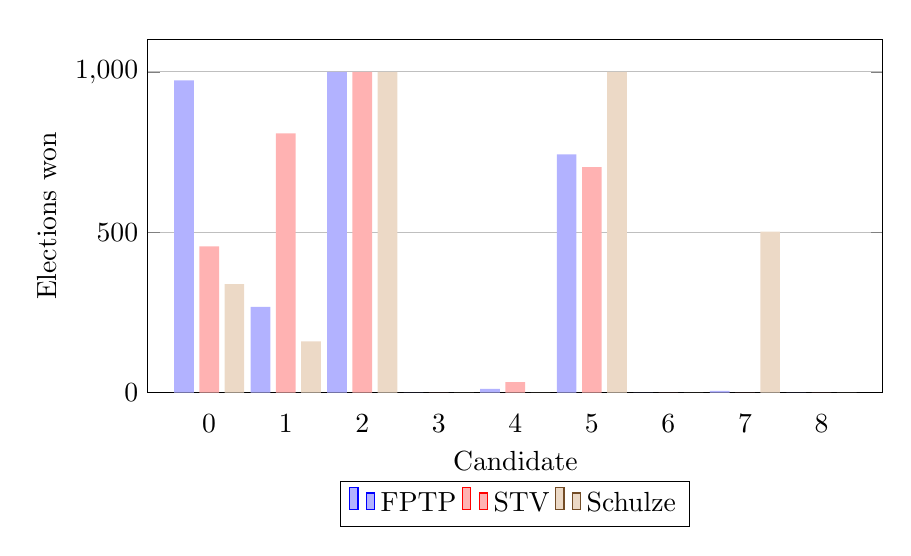
\begin{tikzpicture}
		\begin{axis}[
			ybar,
			width = 0.9\textwidth,
			height = 0.5\textwidth,
			legend style={at={(0.5,-0.25)},
			anchor=north,legend columns=-1},
      x tick style = transparent,
			ylabel = {Elections won},
			xlabel = {Candidate},
			ymajorgrids = true,
			every axis plot/.append style={draw=none,fill,no markers},
      ymin = 0,
			symbolic x coords={0,1,2,3,4,5,6,7,8},
			bar width=0.25cm
      ]
			\addplot coordinates
			{(0, 973)(1, 267)(2, 1000)(3, 0)(4, 12)(5, 743)(6, 0)(7, 5)(8, 0)};
			\addplot coordinates
			{(0, 456)(1, 808)(2, 1000)(3, 0)(4, 33)(5, 703)(6, 0)(7, 0)(8, 0)};
			\addplot coordinates
			{(0, 338)(1, 160)(2, 1000)(3, 0)(4, 0)(5, 1000)(6, 0)(7, 502)(8, 0)};
			\legend{FPTP, STV, Schulze}
		\end{axis}
	\end{tikzpicture}
	\caption{Results in scenario 2}
	\label{fig:scenario 2 result}
\end{figure}

\begin{table}
\centering
\caption{Key metrics for result in scenario 2}
\label{tab:scenario 2 result}
\begin{tabular}{@{}lccc@{}}
\toprule
Method & Standard deviation & Misrepresentation & Most likely winners \\ \midrule
FPTP & 418 & 42\% & 0, 2 \& 5 \\
STV & 388 & 14\% & 1, 2 \& 5 \\
Schulze & 393 & 67\% & 2, 5 \& 7  \\ \bottomrule
\end{tabular}
\end{table}
% [ 418.13628234977, 388.17206952015, 393.25535950293 ]
\subsection{Scenario 3}
Scenario 3 featured 9 candidates of which 3 were to be elected. The distribution of votes was steep. This can be seen by the first-preference votes in figure \ref{fig:example of scenario 3}. The results obtained with each method in this scenario are practically identical. From this, it can be inferred that the results of the methods converge as the preferences in a population become more clear. The results obtained in this scenario can be seen in figure \ref{fig:scenario 3 result}. The key metrics can be found in table \ref{tab:scenario 3 result}.
\begin{figure}[H]
	\centering
	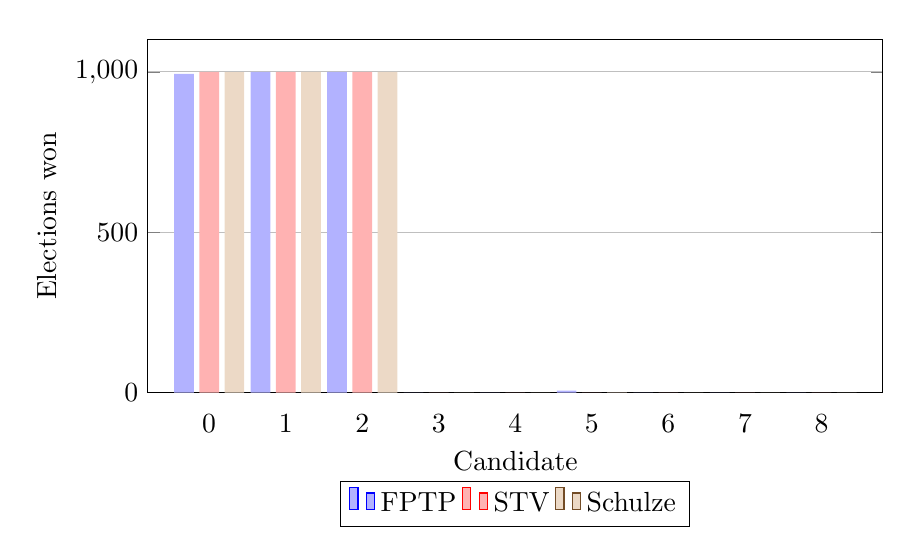
\begin{tikzpicture}
		\begin{axis}[
			ybar,
			width = 0.9\textwidth,
			height = 0.5\textwidth,
			legend style={at={(0.5,-0.25)},
			anchor=north,legend columns=-1},
      x tick style = transparent,
			ylabel = {Elections won},
			xlabel = {Candidate},
			ymajorgrids = true,
			every axis plot/.append style={draw=none,fill,no markers},
      ymin = 0,
			symbolic x coords={0,1,2,3,4,5,6,7,8},
			bar width=0.25cm
      ]
			\addplot coordinates
			{(0, 994)(1, 1000)(2, 1000)(3, 0)(4, 0)(5, 6)(6, 0)(7, 0)(8, 0)};
			\addplot coordinates
			{(0, 1000)(1, 1000)(2, 1000)(3, 0)(4, 0)(5, 0)(6, 0)(7, 0)(8, 0)};
			\addplot coordinates
			{(0, 999)(1, 1000)(2, 1000)(3, 0)(4, 0)(5, 1)(6, 0)(7, 0)(8, 0)};
			\legend{FPTP, STV, Schulze}
			\end{axis}
	\end{tikzpicture}
	\caption{Results in scenario 3}
	\label{fig:scenario 3 result}
\end{figure}

\begin{table}[H]
	\centering
	\caption{Key metrics for result in scenario 3}
	\label{tab:scenario 3 result}
	\begin{tabular}{@{}lccc@{}}
		\toprule
		Method & Standard deviation & Misrepresentation & Most likely winners \\ \midrule
		FPTP & 470 & 33\% & 0, 1 \& 2 \\
		STV & 471 & 33\% & 0, 1 \& 2 \\
		Schulze & 471 & 33\% & 0, 1 \& 2  \\ \bottomrule
	\end{tabular}
\end{table}
Proportionalities: 1:67,7,9 2:42,14,67, 3:33,33,33

\section{Conclusion}
The results obtained in the three different scenarios provide some insight into the varying properties of the different voting systems. Each of the scenarios showed different behaviors for the different methods. For instance, the methods provided practically the same result in scenario 3 but wildly varying results in scenario 2. While the testing method used in this paper may not have been the most robust way of comparing the voting methods, several conclusions can be drawn from the data. I outline them in 4 points below.
\begin{itemize}
	\item Schulze did not seem like a proportional voting method in multi-seat elections.
	\item In single-seat elections, Schulze and STV (and IRV in extension) seemed to provide similar results.
	\item FPTP did not seem like a very proportional method in close elections.
	\item STV seems to be the most proportional method out of the 3 tested, but is not without its flaws.
\end{itemize}
Summary:
There is no perfect voting system. Generally, if you want proportional representation (which in a democracy you want), STV will likely be the best method to use out of the methods covered in this paper.
Modeling of data needs more work, as well as including other methods (such as ...). More research is needed.

\pagebreak

\printbibliography

\section{Appendix}
First-past-the-post program

\end{document}
